\documentclass{article}
\usepackage[utf8]{inputenc}
\usepackage[russian]{babel}
\usepackage{graphicx}
\usepackage{amsmath}
\usepackage{breqn}
\usepackage{wrapfig}
\usepackage{float}
\usepackage{multirow}
\usepackage{caption}
\usepackage{subcaption}

\graphicspath{ {./data/images} }
\author{Александр Романов Б01-107}
\date{}
\title{4.3.1 Изучение дифракции света}

\begin{document}
\maketitle
\section{Введение}
\subsection{Цель работы}
Исследовать явления дифракции Френеля и Фраунгофера на щели, изучить влияние дифракции
на разрешающую способность оптических инструментов.
\subsection{В работе используются}
оптическая скамья, ртутная лампа, монохроматор, щели с регулируемой шириной, рамка с вертикальной
нитью, двойная щель, микроскоп на поперечных салазках с микрометрическим винтом, зрительная труба.
\section{Работа}
\subsection{Дифракция Френеля на щели}
\subsubsection{Подготовка}
Определим нуль микрометрического винта \(S_2\). Глядя сквозь щель на лампу определим момент открытия щели:
\[ l_0 = 0.014\;mm \]
Запишем параметры установки:
\[ f_1 = 12.5\;cm \]
\[ f_2 = 12.5\;cm \]
\[ \lambda = 5461\;\text{\AA} \]


\begin{figure}[H]
  \centering
  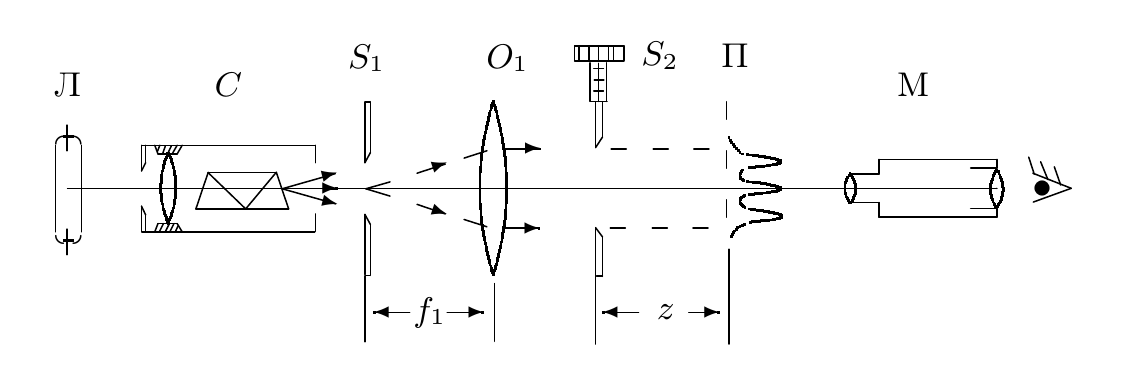
\includegraphics[width=\textwidth]{frnl-scheme.png}
  \caption{Схема установки для наблюдения дифракции Френеля}
  \label{fig:frnl}
\end{figure}

Соберём схему с Рис.\ref{fig:frnl}.

Откроем щель пошире и с помощью листа бумаги убедимся что свет идёт вдоль оптической скамьи.

Установим линзу \(O_1\) на расстоянии от \(S_1\) близком к фокусному \(F_2 = 12.5\;cm\). Точно настроим пучок на параллельность
с помощью зрительной трубы.

Установим ширину щели \(S_2\) в \(b = 0.33\;mm\) и поставим за линзой \(O_1\).

Сфокусируем микроском на щели \(S_2\). Перемещая его вдоль оптической скамби получим резкое изображение щели.
Видно также что при небольшом удалении микроскопа от щели на ярком фоне изображения щели
появляются узкие тёмные полосы.
\subsubsection{Измерения}
Снова получим резкое изображение щеи в микроскопе (\(x_0 = 45.3\;cm\)).
Получим в микроскопе 1 тёмную полосу \(x_1 = 46.6\;cm \Rightarrow z = 1.3\;cm\)

Снимем зависимость координаты микроскопа отчисла \(n\) наблюдаемых тёмных полос.

\begin{table}[H]
  \centering
  \begin{tabular}{|c|c|c|c|c|c|}
    \hline
   \(n\)        &   1  &   2  &   3  &   4  &   5    \\\hline
   \(x_n, cm\)  & 46.6 & 46.2 & 45.9 & 45.7 & 45.6 \\\hline
   \(z_n, cm\)  & 1.3  & 0.9  & 0.6  & 0.4  & 0.3 \\\hline
  \end{tabular}
\end{table}

Открыв щель \(S_2\) шире и сдвинув микроскоп наблюдаем дифракцию на краю экрана.

Заменив щель на нить наблюдаем дифракцию на препядствии.

\subsubsection{Обработка результатов}
Расчитаем зоны Френеля по формуле:
\[ \xi_n = \sqrt{z_nn\lambda} \]

\begin{table}[H]
  \centering
  \begin{tabular}{|c|c|c|c|c|c|}
    \hline
   \(n\)              &  1  & 2   &  3  &  4  &  5    \\\hline
   \(2\xi_n, \mu m\)  & 168 & 198 & 198 & 186 & 181   \\\hline
  \end{tabular}
\end{table}

Построим график:
\begin{figure}[H]
  \centering
  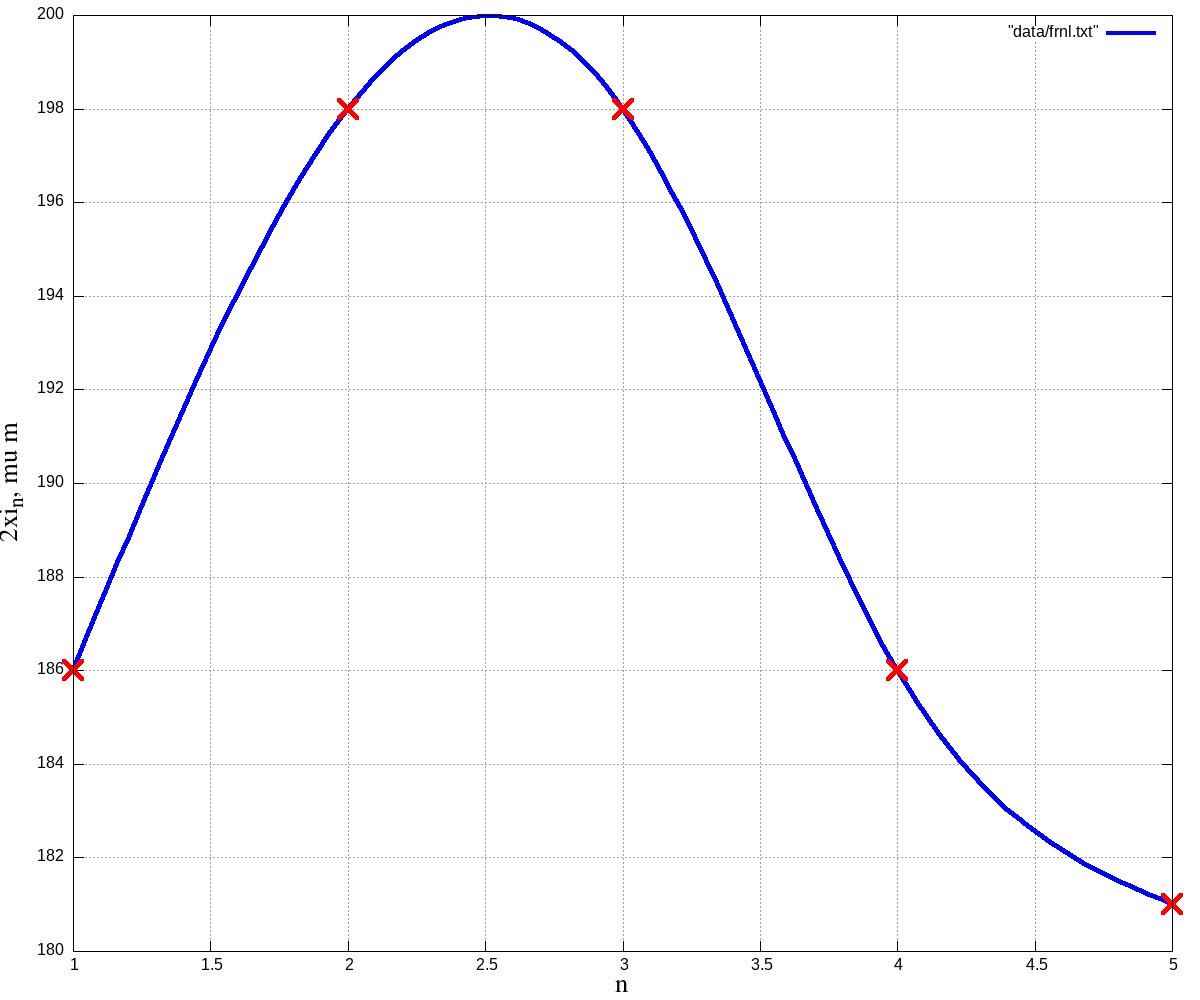
\includegraphics[width=\textwidth]{frnl.png}
\end{figure}

\subsection{Дифракция Фраунгофера на щели}
\begin{figure}[H]
  \centering
  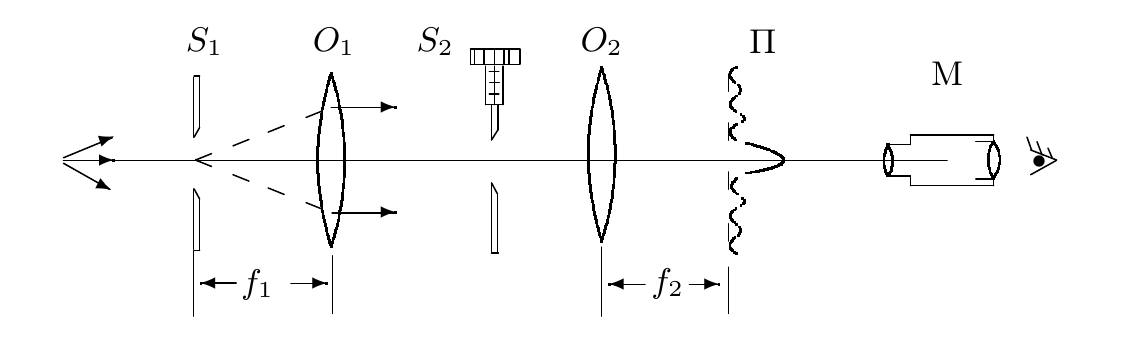
\includegraphics[width=\textwidth]{fgfr-scheme.png}
  \caption{Схема установки для наблюдения дифракции Фраунгофера}
  \label{fig:fgfr}
\end{figure}

Соберём схему с Рис.\ref{fig:fgfr}.

Настроим микроскоп на фокальную плоскость линзы и поставим между ними щель \(S_2\).
Изменением её ширины добьёмся появления дифракционной картины.

Измерим с помощью шкалы микроскопа координаты \(x_m\) нескольких дифракционных минимумов:

\begin{table}[H]
  \centering
  \begin{tabular}{|c|c|c|c|c|c|}
    \hline
   \(n\)           &  1    & 2     &  3    &  4    &  5    \\\hline
   \(x_n,\;mm\)    & 0.120 & 0.088 & 0.056 & 0.024 & 0.000 \\\hline
  \end{tabular}
\end{table}

Построим график:
\begin{figure}[H]
  \centering
  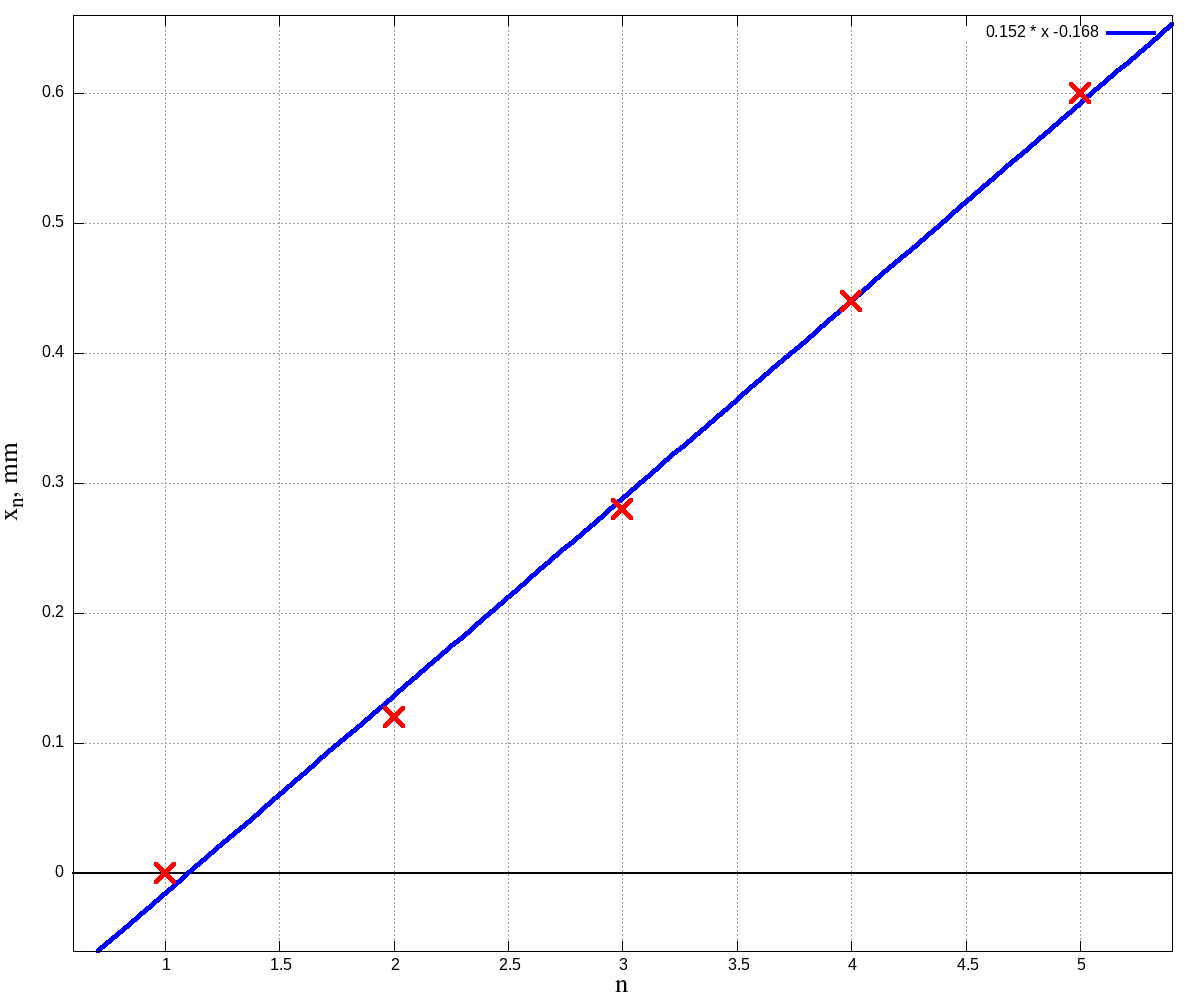
\includegraphics[width=0.8\textwidth]{fgfr.png}
\end{figure}
Полученная зависимость вида \(x_n = kn + b\):
\[ k = (-0.030 \pm 0.001)\;mm \]
\[ b = (0.149 \pm 0.001)\;mm \]

Итого среднее расстояние \(\Delta x\) между соседними минимумами:
\[ \Delta x = (0.030 \pm 0.001)\; mm \]
При этом из формулы:
\[ x_m = m \frac{\lambda}{b}f_2 \]
вычислим значение b:
\[ b = \frac{\lambda f_2}{k} = (2.2 \pm 0.0)\;mm\]
Это значение на порядок отличается от реального \(b = 0.34\;mm\)

\subsection{Дифракция Фраунгофера на двух щелях}
Не перемещая линз и микроскопа заменим щель \(S_1\) на щель \(S_2\) и найдём резкое изображение.
На бывшее место \(S_2\) поставим поставим экран с двойной щелью. Итого как на Рис. \ref{fig:fgfr2}:
\begin{figure}[H]
  \centering
  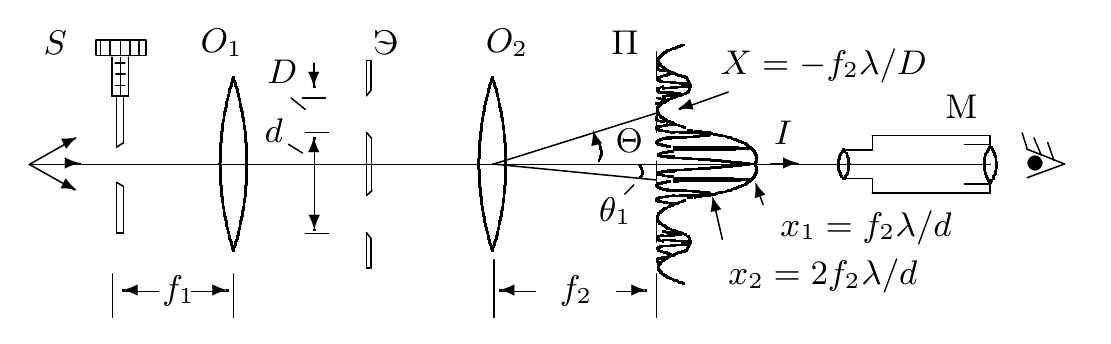
\includegraphics[width=\textwidth]{fgfr-scheme-2.png}
  \caption{Схема установки для наблюдения дифракции Фраунгофера на 2 щелях}
  \label{fig:fgfr2}
\end{figure}

\subsubsection{}
Определим с помощью шкалы микроскопа растояние между самыми удалёнными друг от друга тёмными полосами
внутри центрального максимума:
\[ l = (0.14 \pm 0.02)\;mm \]
Число светлых промежутков между ними:
\[ N = 8\pm 0 \]
Определим расстояние \(\delta x\) между соседними минимумами:
\[ \delta x = \frac{l}{N} = (0.018\pm 0.003)\; mm \]

Определим расстояние между щелями \(d\) по формуле:
\[ \delta x = f_2\frac{\lambda}{d} \]
\[ d = f_2\frac{\lambda}{\delta x} = (3.8\pm 0.6)\;mm \]

Измерив то же расстояние с помощью микроскопа:
\[ d = (0.84\pm 0.02)\;mm \]
Значения снова разошлись на 1 порядок.

\subsubsection{}
Расширяя входную щель определим её размер при котором наступает первое исчезновение интерференционных полос:
\[ b_0 = (0.08\pm 0.01)\;mm \]

Теперь получим значение \(b_0\) из формулы:
\[ \frac{b_0}{f_1} = \frac{\lambda}{d} \Rightarrow b_0 = f_1\frac{\lambda}{d} = (0.008 \pm 0.002\;mm)\]
Значения и сейчас разошлись на порядок.

\section{Выводы}
В ходе выполнения работы:
\begin{enumerate}
  \item Были изучены различные виды дифракции: Френеля, и Фраунгофера на щели и на двух щелях.
  \item Были измерены различные параметры установки:
  \[ b = (2.2 \pm 0.0)\;mm \]
  \[ b_0 = (0.08\pm 0.01)\;mm \]
  \[ d = (3.8\pm 0.6)\;mm \]
  Все эти величины оказались на 1 порядок больше измеренных напрямую. Это может говорить как о неточности измерений
  (В ходе выполнения работы часто тяжело было понять сколько именно интерференционных полос видно и когда они 
  начинают исчезать), так и об ошибках в последующих вычислениях, которых мне обнаружить не удалось.
\end{enumerate}

\end{document}